\documentclass[a4 paper]{article}
\usepackage[inner=2.0cm,outer=2.0cm,top=2.5cm,bottom=2.5cm]{geometry}
\usepackage{setspace}
\usepackage[rgb]{xcolor}
\usepackage{verbatim}
\usepackage{subcaption}
\usepackage{amsgen,amsmath,amstext,amsbsy,amsopn,tikz,amssymb}
\usepackage{fancyhdr}
\usepackage[colorlinks=true, urlcolor=blue,  linkcolor=blue, citecolor=blue]{hyperref}
\usepackage[colorinlistoftodos]{todonotes}
\usepackage{rotating}
\usepackage{booktabs}
\newcommand{\ra}[1]{\renewcommand{\arraystretch}{#1}}


\newtheorem{thm}{Theorem}[section]
\newtheorem{prop}[thm]{Proposition}
\newtheorem{lem}[thm]{Lemma}
\newtheorem{cor}[thm]{Corollary}
\newtheorem{defn}[thm]{Definition}
\newtheorem{rem}[thm]{Remark}
\numberwithin{equation}{section}

\newcommand{\homework}[6]{
   \pagestyle{myheadings}
   \thispagestyle{plain}
   \newpage
   \setcounter{page}{1}
   \noindent
   \begin{center}
   \framebox{
      \vbox{\vspace{2mm}
    \hbox to 6.28in { {\bf CSE 211:~Discrete Mathematics \hfill {\small (#2)}} }
       \vspace{6mm}
       \hbox to 6.28in { {\Large \hfill #1  \hfill} }
       \vspace{6mm}
       \hbox to 6.28in { {\it Instructor: {\rm #3} \hfill  {\rm #5} \hfill  {\rm #6}} \hfill}
       \hbox to 6.28in { {\it Assistant: #4  \hfill #6}}
      \vspace{2mm}}
   }
   \end{center}
   \markboth{#5 -- #1}{#5 -- #1}
   \vspace*{4mm}
}

\newcommand{\problem}[2]{~\\\fbox{\textbf{Problem #1}}\hfill (#2 points)\newline\newline}
\newcommand{\subproblem}[1]{~\newline\textbf{(#1)}}
\newcommand{\D}{\mathcal{D}}
\newcommand{\Hy}{\mathcal{H}}
\newcommand{\VS}{\textrm{VS}}
\newcommand{\solution}{~\newline\textbf{\textit{(Solution)}} }

\newcommand{\bbF}{\mathbb{F}}
\newcommand{\bbX}{\mathbb{X}}
\newcommand{\bI}{\mathbf{I}}
\newcommand{\bX}{\mathbf{X}}
\newcommand{\bY}{\mathbf{Y}}
\newcommand{\bepsilon}{\boldsymbol{\epsilon}}
\newcommand{\balpha}{\boldsymbol{\alpha}}
\newcommand{\bbeta}{\boldsymbol{\beta}}
\newcommand{\0}{\mathbf{0}}

\documentclass[tikz,border=10pt]{standalone}
\usetikzlibrary{positioning}
\tikzset{main node/.style={circle,fill=blue!20,draw,minimum size=1cm,inner sep=0pt},
            }


\begin{document}
\homework{Homework \#3}{Due: 03/01/22}{Dr. Zafeirakis Zafeirakopoulos}{Gizem S\"ung\"u}{}{}
\textbf{Course Policy}: Read all the instructions below carefully before you start working on the assignment, and before you make a submission.
\begin{itemize}
\item It is not a group homework. Do not share your answers to anyone in any circumstance. Any cheating means at least -100 for both sides. 
\item Do not take any information from Internet.
\item No late homework will be accepted. 
\item For any questions about the homework, send an email to gizemsungu@gtu.edu.tr
\item The homeworks (both latex, pdf and/or source code files in a zip file) will be
submitted into the course page of Teams.
\item The latex, pdf or source code and zip files of the homeworks should be saved as
"StudentId".$\{$tex, pdf, c, py, cpp, java, zip$\}$.
\item If the answers of the homeworks have only calculations without any formula or any explanation -when needed- will get zero.
\end{itemize}

\problem{1: Relations}{20}
Let $\mathbb{Z}$ be the set of all integers. Define relation R on $\mathbb{N}$ as follows.
\begin{equation*}
	\forall a, b \in \mathbb{N}, (a, b) \in R \text{ iff } \exists i \in \mathbb{Z},  \frac{a}{b} = 2^i
\end{equation*}
Prove that R is an equivalence relation. Show your work step by step.
\newline
\newline
Solution : For equivalance relation the relation must be reflexive, symmetric and transitive.
\newline
Reflexivity :  $$\frac{a}{a} = {2^i}  \mbox{  and} $$
               $$ 1 = {2^i} \mbox{  when i = 0}$$
\newline
Symmetric :  $$\frac{a}{b} = {2^i}  \mbox{  and }  a = {2^i}.b  $$
             $$\frac{b}{a} = {2^i} \mbox{  and  }  b = {2^i}.a  $$
             $$ 2^{2i} = 1   \mbox{     when i = 0} $$
\newline
Transitive:  $$ \mbox{for (a, b)  =   } \frac{a}{b} = {2^i}  \mbox{  and} $$
             $$ \mbox{for (b, c)  =   } \frac{b}{c} = {2^i}  \mbox{  and} $$
             $$ \mbox{for (a, c)  =   } \frac{a}{c} = {2^i}   $$
             $$ \mbox{for use all of these equations we get   }$$
             $$ {2^i} = 1   \mbox{     when i = 0}  $$
\newline
\problem{2: Relations}{15}
Define he relation R on $\mathbb{N}$ as 
\begin{equation*}
	\forall c, d \in \mathbb{N}, (c, d) \in R \text{ iff } c+d \text{ is even.}
\end{equation*}
\subproblem{a} Prove that R is an equivalence relation.
\newline
Solution : For equivalance relation the relation must be reflexive, symmetric and transitive.
Reflexivity :  $$\mbox{ c+c = 2c  (even)} $$
Symmetric :  $$\mbox{ c+d = 2n and} $$
             $$\mbox{ d+c = 2n so it is even} $$
Transitive:  $$ \mbox{for (c, d)  =   } \mbox{ c+d = 2n   and} $$
             $$ \mbox{for (d, f)  =   } \mbox{ d+f = 2k  and} $$
             $$ \mbox{for (c, f)  =   } \mbox{ c+f = 2n-d+2k-d = 2n+2k-2d = 2(n+k-d)  so it is even} $$
\subproblem{b} How many equivalence classes does R have?
\newline
[1] = {1,3,5,7,9....}   and  [3] = {1,3,5,7,9....}
\newline
[2] = {2,4,6,8,10...}   and  [4] = {2,4,6,8,10....}
\newline
For all of these equations we can say there are two different type of equivalence classes.
\problem{3: Relations}{10}
Let R and S be two relations both on A. Show that
\subproblem{a} If R and S are both reflexive, is R $\cap$ S also reflexive?
\newline
\newline
Solution:
\newline
(a,a) \in R, (a,a) \in S
\newline
\forall a \in A (a,a)  \in R $\cap$ S   \mbox{  so that R $\cap$ S is reflexive}
\newline
\subproblem{b} If R and S are both symmetric, is R $\cap$ S also symmetric?
\newline
\newline
Solution:
\newline
(a,b), (b,a) \in R, (a,b), (b,a)\in S
\newline
(a,b), (b,a)\in R $\cap$ S   \mbox{  so that R $\cap$ S is symmetric}
\newline
\subproblem{c} If R and S are both transitive, is R $\cap$ S also transitive?
\newline
\newline
Solution:
\newline
(a,b), (b,a), (a,c)\in R, (a,b), (b,a), (a,c)\in S
\newline
(a,b), (b,a), (a,c)\in R $\cap$ S   \mbox{  so that R $\cap$ S is transitive}
\newline
\newline
Note: Of course, yes or no answers are not acceptable. Show your work briefly.
\newpage
\problem{4: Relations}{15}
Give a poset that has
\subproblem{a} a minimal element but no maximal element.
\newline
Solution:
\newline
($\mathbb{N}$, $\leq$)  $\mbox{   minimal element = 0 but no maximal element.}$
\subproblem{b} a maximal element but no minimal element.
\newline
Solution:
\newline
($\mathbb{Z^-}$, $\leq$)  $\mbox{   maximal element is -1 but no minimal element.}$
\subproblem{c} neither a maximal nor a minimal element.
\newline
Solution:
\newline
($\mathbb{Z}$, $\leq$)  $\mbox{   neither a maximal nor a minimal element.}$

\problem{5: Relations}{15}
Suppose that (S, $\preccurlyeq_1$) and (T , $\preccurlyeq_2$) are posets. Show that
(S $\times$ T , $\preccurlyeq$) is a poset where (s, t) $\preccurlyeq$ (u, v) if and only if
s $\preccurlyeq_1$ u and t $\preccurlyeq_2$ v. Show your work in details. 
\newline
Solution:
\newline
k,l $\in$ S   means  k $\preccurlyeq_1$ l
\newline
m,n $\in$ T   means  m $\preccurlyeq_2$ n
\newline
(k,m) $\preccurlyeq$  (k,n)
\newline
(k,m) $\preccurlyeq$  (l,n)
\newline
(k,m) $\preccurlyeq$  (l,m)
\newline
S × T = {(k,m), (l,m), (k,n), (l,n)} so is a poset

\problem{6: Relations}{10}
Answer these questions for the partial order represented by this Hasse diagram.
\begin{figure}[htb]
	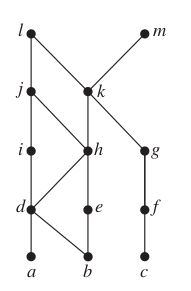
\includegraphics[scale=0.5]{hasse.png}
\end{figure}
\subproblem{a} Find the maximal elements.
\newline
Solution : l and m
\subproblem{b} Find the minimal elements.
\newline
Solution : a, b and c
\subproblem{c} Is there a greatest element?
\newline
Solution : No. There is not a greatest element.
\subproblem{d} Is there a least element?
\newline
Solution : No. There is not a least element.
\subproblem{e} Find all upper bounds of $\{a, b, c\}$.
\newline
Solution : k, l and m
\subproblem{f} Find the least upper bound of  $\{a, b, c\}$, if it exists.
\newline
Solution : k 
\subproblem{g} Find all lower bounds of  $\{f, g, h\}$.
\newline
Solution : There is not exist. 
\subproblem{h} Find the greatest lower bound of  $\{f, g, h\}$, if it exists.
\newline
Solution : There is not exist. 
\newline
\newline
\newline
\problem{7: Graphs}{10}
Determine whether the directed graph shown has an Euler circuit. Construct an Euler circuit if one exists. If no Euler circuit exists, determine whether the directed graph has an Euler path. Construct an Euler path if one exists.
\subproblem{a}
\begin{figure}[htb]
	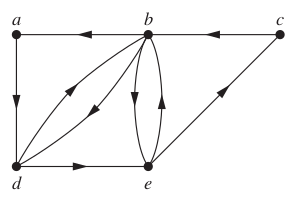
\includegraphics[scale=0.5]{euler.png}
\end{figure}
\newline
Solution: In the graph; indegree and outdegree of each vertex are same.
And every vertex pairs meet. So this graph has an Euler circuit.
\newline
Euler circuit: a, d, b, d, e, b, e, c, b, a
\subproblem{b}
\begin{figure}[h]
	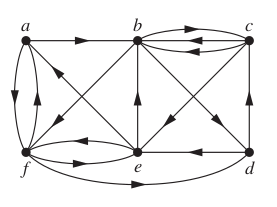
\includegraphics[scale=0.5]{euler2.png}
\end{figure}
\newline
Solution: For Euler circuit: In the graph; every vertex pairs meet. But indegree and outdegree of each vertex are not same because (c has 2 indegree and 3 outdegree and b has 4 in-degree and 3 out-degree). So this graph has not an Euler circuit.
\newline
For Eular path: In the graph; c has 2 indegree and 3 outdegreethat mean outdegree larger than indegree. And b has 4 indegree and 3 outdegree mean in-degree larger than outdegree. And every vertex pairs meet.
\newline
Euler Path: c, b, c, e, f, e, a, f, a, b, f, d, e, b, d, c, b

\problem{8: Graphs}{25}
Remember graph coloring problem in the problem session.
\subproblem{a} Draw the graph of the following code block.
\newline
Solution:
\newline
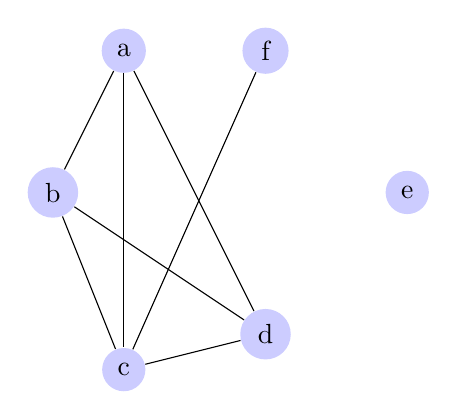
\begin{tikzpicture}  
  [scale=.9,auto=center,every node/.style={circle,fill=blue!20}]   
    
  \node (a1) at (2,5)  {b}; 
  \node (a2) at (3,7)  {a};  
  \node (a3) at (3,2.5) {c};  
  \node (a4) at (5,7)  {f};  
  \node (a5) at (5,3)  {d};  
  \node (a6) at (7,5)  {e};  
  
  \draw (a2) -- (a1);
  \draw (a2) -- (a3);
  \draw (a2) -- (a5);
  \draw (a1) -- (a3);
  \draw (a1) -- (a5);
  \draw (a3) -- (a5);
  \draw (a3) -- (a4);
  
\end{tikzpicture}  
  
\subproblem{b} Explain how you represent the components of the code in graph coloring problem. 
\newline
Solution: Values that need to be kept in memory at the same time cannot get the same register.
\newline
\subproblem{c} What is the minimum number of registers that you need to compile the code? Show which variables can be in the same register.
\newline
Solution: 
\newline
Minimum number of registers are 4.
\newline
Register 1: a
\newline
Register 2: b
\newline
Register 3: c
\newline
Register 4: d, e, f
\newline


\begin{itemize}
	\item[Line 1:] a = 3
	\item[Line 2:] b = 6
	\item[Line 3:] c = 4
	\item[Line 4:] d = b + c
	\item[Line 5:] e = d + a
	\item[Line 6:] if e $<$ 4 then f = 4 $\times$ b   
	\item[Line 7:] else then f = 6 $\times$ a
	\item[Line 8:] d = f - c
\end{itemize}

\problem{9: Graphs}{10}
Draw graphs which are given in adjaceny matrices as follows. Explain if these graphs are isomorphic?


\begin{equation*}
G_1 = \begin{bmatrix} 
0 & 1 & 0 & 1\\
1 & 0 & 0 & 1\\
0 & 0 & 0 & 1\\
1 & 1 & 1 & 0
\end{bmatrix}\mbox{ ~    ~ }     
G_2 = \begin{bmatrix}
0 & 1 & 1 & 1\\
1 & 0 & 0 & 1\\
1 & 0 & 0 & 1\\
1 & 1 & 1 & 0
\end{bmatrix}
\end{equation*} 
\newline
Solution:
\newline
G1 = 
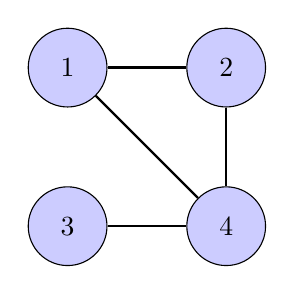
\begin{tikzpicture}
    \begin{scope}[xshift=4cm]
    \node[main node] (1) {$1$};
    \node[main node] (2) [right = 1cm  of 1]  {$2$};
    \node[main node] (3) [below = 1cm  of 1] {$3$};
    \node[main node] (4) [right = 1cm  of 3] {$4$};

    \path[draw,thick]
    (1) edge node {} (2)
    (1) edge node {} (4)
    (2) edge node {} (4)
    (3) edge node {} (4)
    ;
    \end{scope}
\end{tikzpicture}
\newline
\newline
  G2 = 
\begin{tikzpicture}
    \begin{scope}[xshift=4cm]
    \node[main node] (4) {$4$};
    \node[main node] (5) [right = 1cm  of 1]  {$5$};
    \node[main node] (6) [below = 1cm  of 1] {$6$};
    \node[main node] (7) [right = 1cm  of 3] {$7$};

    \path[draw,thick]
    (4) edge node {} (5)
    (4) edge node {} (6)
    (4) edge node {} (7)
    (5) edge node {} (7)
    (6) edge node {} (7)
    ;
    \end{scope}
\end{tikzpicture}
\newline
These graphs are not isomorphic because number of edges are different each other.


\end{document} 
